\documentclass[11pt]{article}
\usepackage[margin=1in]{geometry}
\usepackage{amsmath,amssymb,booktabs,graphicx,setspace,caption,hyperref}
\usepackage[T1]{fontenc}
\usepackage{mathpazo}
\setlength{\parindent}{0pt}
\setlength{\parskip}{0.6em}
\captionsetup{font=small,skip=6pt}
\title{Panel MS-AR(1) for EMBI countries from 1990\\[0.4em]\large Seasonally adjusted real GDP per worker}
\author{}
\date{}
\begin{document}
\maketitle
\section{Model}
Countries that are in the J.P.\ Morgan EMBI Global as of April 2025, or that appear on an earlier published EMBI Global coverage list (Korea, Thailand, Croatia, and Tunisia). Of that list, 43 countries are in the 2026-09-17 panel. The three with the lowest 2019 real GDP per worker are dropped (KEN, CMR, BOL). Estimation starts in 1990.
One specification. Joint panel Markov-switching AR(1) around a common linear trend, with Normal random intercepts. No catch-up term.
\begin{align}
y_{it} &= a_i + g\, t + z_{it}, \\
a_i &\sim \mathcal{N}(\alpha,\omega^2), \\
z_{i,t+1} &= \bigl(1-\rho(s_{it})\bigr)\mu(s_{it}) + \rho(s_{it})\, z_{it} + \sigma(s_{it})\,\varepsilon_{it}, \\
s_{i,t+1} &\sim \Pi(\,\cdot\mid s_{it}).
\end{align}
Outcome is log seasonally adjusted real GDP per worker. Three regimes. The unconditional mean of the cycle is restricted to $E[z]=0$ (the median regime mean is not pinned at 0). $\sigma$ and $\rho$ switch. $|\rho|<0.99$. Random intercepts use 11-point Gauss--Hermite. Plotted cycles use the posterior mean of $a_i$. Standard errors are delta-method from a numerical Hessian.
\clearpage
\section{EMBI countries from 1990, three poorest in 2019 dropped}
EMBI subsample of the 2026-09-17 SA panel from 1990, dropping KEN, CMR, BOL (lowest 2019 real GDP per worker). $y_{it}=a_i+gt+z_{it}$, $E[z]=0$. 40 countries, 4051 observations, 1990-Q1--2026-Q2. Fitted countries: 40. Observations: 4051. Log-likelihood: 9966.60.
Random intercepts $a_i\sim N(\alpha,\omega^2)$ with $\alpha=-5.5522$ (0.0490), $\omega=0.6129$ (0.0213). Posterior-mean $a_i$: mean -5.653, min -6.702, max -4.402. Common slope $g=0.0088$ (0.0011).
\begin{table}[h]
\centering
\caption{Regime AR(1), transition matrix, and ergodic $\pi$. Columns are regimes.}
\begin{tabular}{lccc}
\toprule
 & (0) & (1) & (2) \\
\midrule
$\mu$ & -0.9632 & -0.1565 & 0.3453 \\
 & (0.1827) & --- & (0.0343) \\ \addlinespace
$\sigma$ & 0.0948 & 0.0230 & 0.0087 \\
 & (0.0055) & (0.0008) & (0.0003) \\ \addlinespace
$\rho$ & 0.9900 & 0.9900 & 0.9899 \\
 &  & (0.0000) & (0.0003) \\ \addlinespace
$\Pi_{0\cdot}$ & 0.5593 & 0.4070 & 0.0337 \\
 & (0.0581) & (0.0604) & (0.0222) \\ \addlinespace
$\Pi_{1\cdot}$ & 0.0636 & 0.8721 & 0.0643 \\
 & (0.0102) & (0.0151) & (0.0109) \\ \addlinespace
$\Pi_{2\cdot}$ & 0.0060 & 0.0727 & 0.9213 \\
 & (0.0052) & (0.0114) & (0.0099) \\ \addlinespace
$\pi$ & 0.0766 & 0.4903 & 0.4331 \\
 & (0.0115) & (0.0302) & (0.0342) \\ \addlinespace
\bottomrule
\end{tabular}
\end{table}
\begin{figure}[h]
\centering
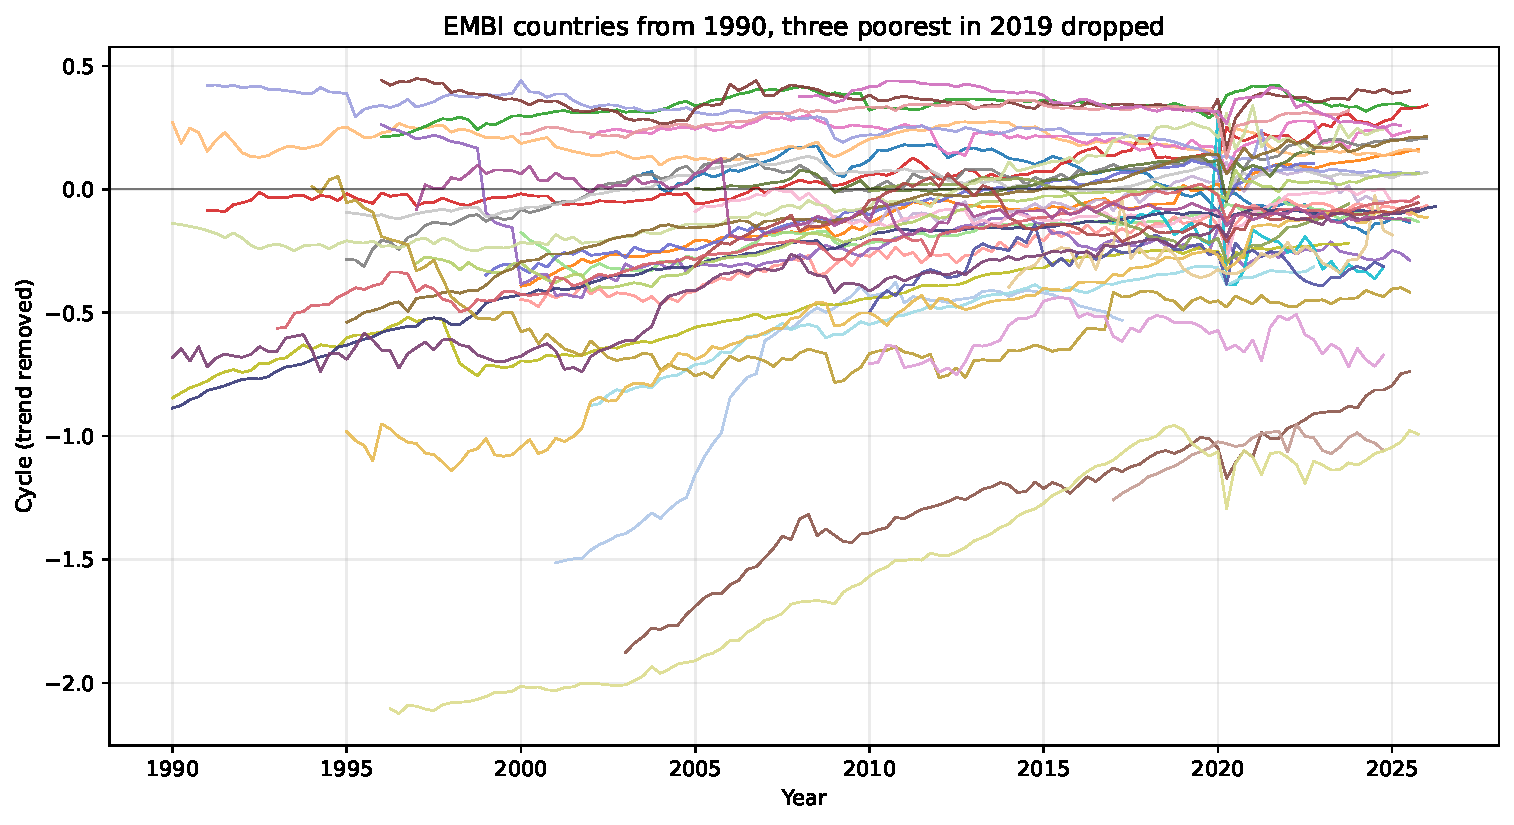
\includegraphics[width=0.75\textwidth]{figs/cycle_embi_1990.pdf}
\caption{Country cycles after removing the posterior-mean intercept and the common linear trend.}
\end{figure}
\end{document}
